\documentclass[12pt]{article}

% Packages
\usepackage{graphicx}
\usepackage{amsmath}
\usepackage{amsfonts}
\usepackage{amssymb}
\usepackage[letterpaper,top=2cm,bottom=2cm,left=3cm,right=3cm,marginparwidth=1.75cm]{geometry}
\usepackage{minted}
\usepackage{rotating}
\usepackage{pdflscape}
\usepackage{csvsimple}
\usepackage{pgfplotstable}
\usepackage{multicol}
\usepackage{supertabular}
\usepackage{booktabs}
\usepackage{longtable}
\pgfplotsset{compat=newest}

\makeatletter
\let\mcnewpage=\newpage
\newcommand{\TrickSupertabularIntoMulticols}{%
\renewcommand\newpage{%
    \if@firstcolumn%
        \hrule width\linewidth height0pt%
            \columnbreak%
        \else%
          \mcnewpage%
        \fi%
}%
}
\makeatother



% Title page
\title{Hand in problem 2 in Information Theory}
\author{Fredrick Nilsson}
\date{\today}

\begin{document}

\maketitle

\newpage

\section*{Report}

\begin{landscape}
    \begin{figure}
        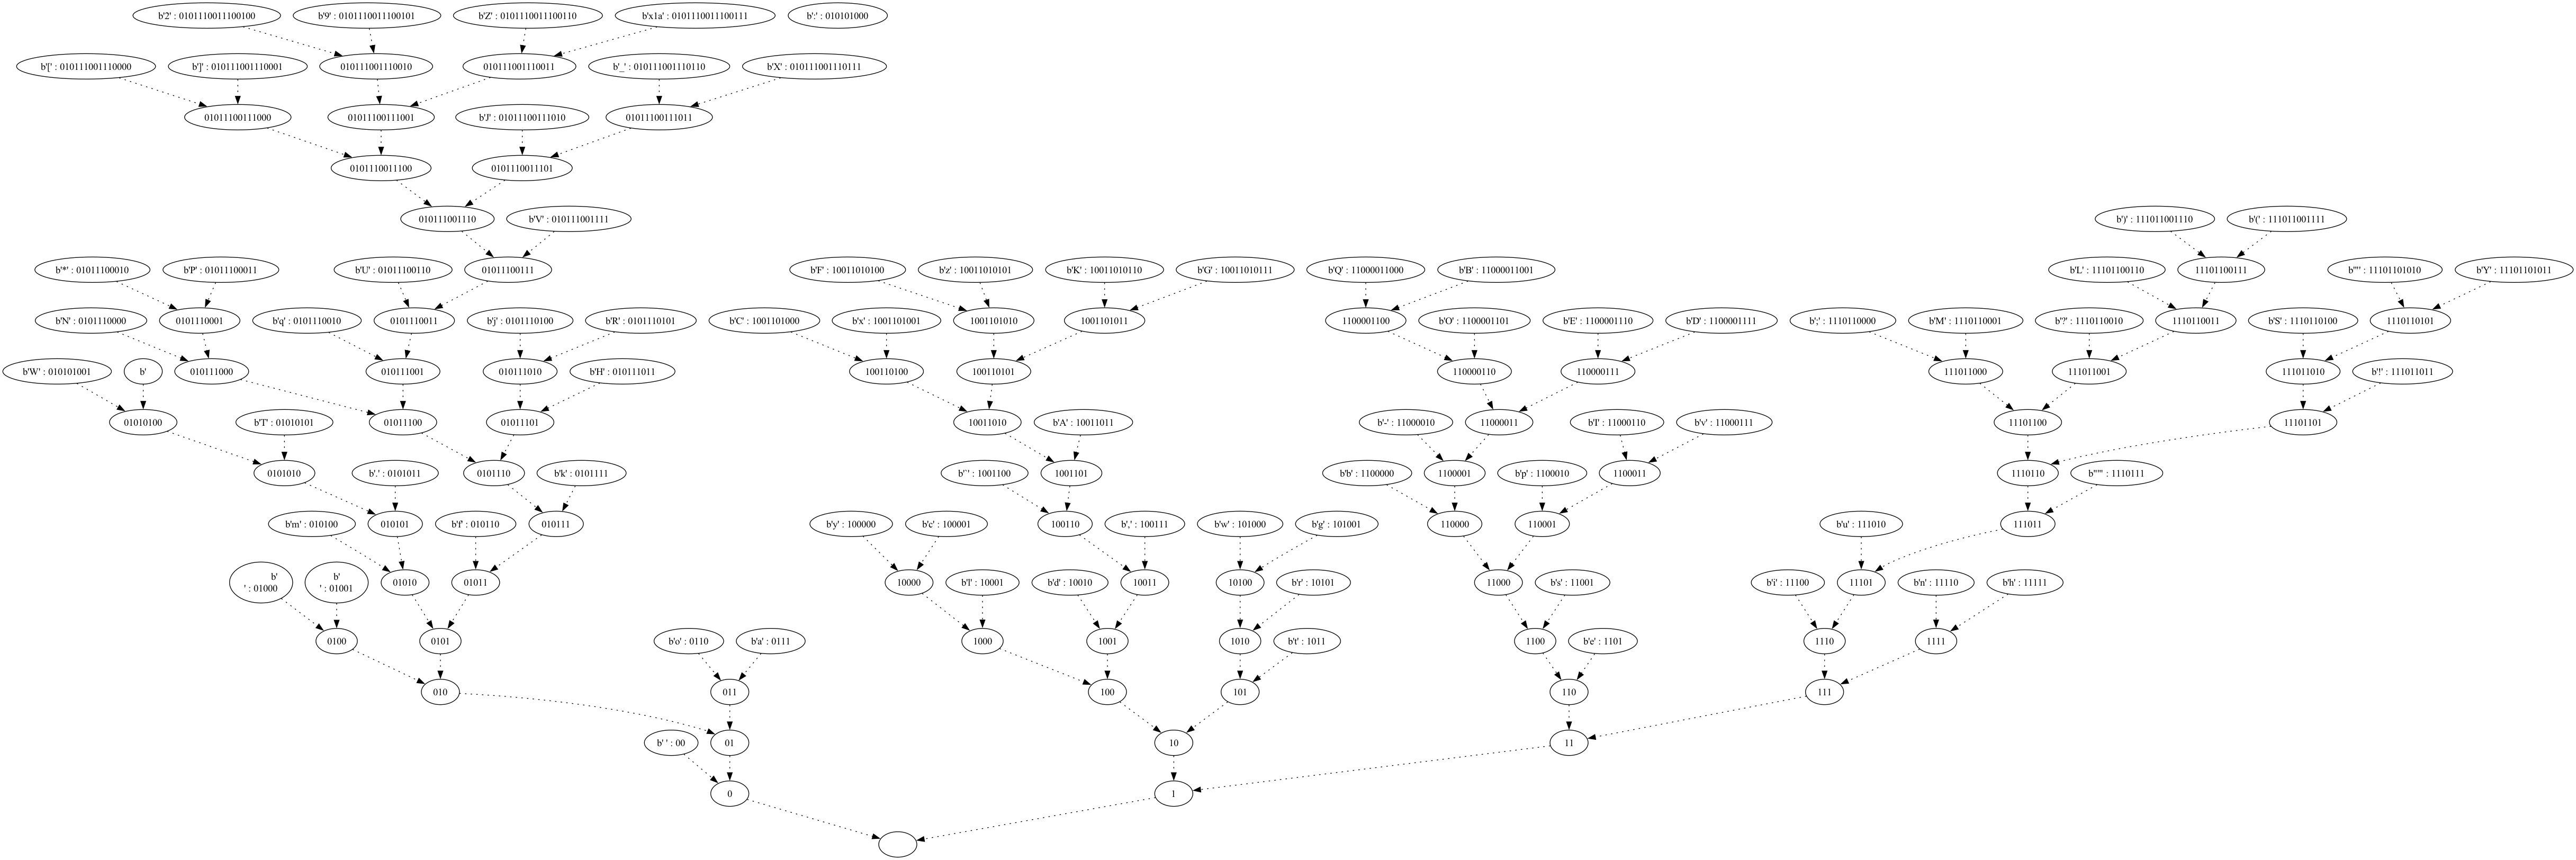
\includegraphics[width=1.6\textwidth]{../postorder_traversal.png}
        \caption{The huffman tree}
        \label{fig:tree}
    \end{figure}
\end{landscape}

\section*{Source code}
\inputminted[breaklines]{python}{../handin.py}

\newpage
\section*{Codebook}

\newbox\myb
\setbox\myb\vbox{\hsize=\dimexpr(\textwidth-\columnsep)/2\relax
\makeatletter
\chardef\LT@end@pen\z@
\makeatother
\begin{longtable}{lll}
    \toprule
    \textbf{Ascii} & \textbf{Count} & \textbf{Code}\\
    \midrule
    \endhead
    \bottomrule
    \endfoot
    \csvreader[
        late after line=\\,
        respect all,
        ]
    {../code_table.csv}{symbol=\symbol,probability=\probability,code=\code}{\symbol & \probability & \code}
\end{longtable}}
\begin{multicols*}{2}
\unvbox\myb
\end{multicols*}
\end{document}
